\documentclass[11pt,en]{elegantpaper}
\usepackage{float}
\title{Privacy-Preserving Protocol Based On Bluetooth Encrypted Data Sharing}
\author{Wangzhihui Mei 2019124044\ Hongyi Huang 2019180029 \ Zijia He 2019124057 \ Chang Xu 2019180034\\ Tianyu Jin 2019180030 \ Zhanping Zhou 2019124060 \ Senmiao Liu 2019180036 \ Caiming Qian 2019124036}
\institute{CCNU-UOW JI}

\version{}
\date{}


\begin{document}

\maketitle

\begin{abstract}
	At the critical moment of resisting COVID-19, governments and health authorities are working together to find solutions to the COVID‑19 pandemic, to protect people and get society back up and running across the world\cite{guan2020clinical} . Given the widespread use of "health codes", this paper proposes a more reasonable privacy-preserving protocol based on Bluetooth data sharing. It is mainly constructed from short-distance Bluetooth low energy beacon data-transmission and some encryption methods.
\end{abstract}

\section{Introduction}
At present, new coronavirus is rampant around the world, and the whole world is facing a massive challenge. Even if medical technology is quite developed, the new coronavirus discovered for the first time in large-scale infections are still somewhat helpless.

Fortunately, China has found a suitable and reasonable way to resist COVID-19, in which the government take severe administrative measures to keep distance between citizens. To effectively control the epidemic, China has not only continuously developed vaccines from the technical aspect but also adopted a powerful political means: isolation. Quarantine dramatically reduces the spread of the epidemic. Then,  the economy and society need to recover to regular order. To prevent the virus from spreading again, and better track the infected, accelerate the research of the vaccine, it is essential to develop a reasonable infected tracking system.

The "health code", as a pass for returning personnel, records the individual's health and takes the form of "green code", "red code", and "yellow code" to detect data dynamically. The appearance of the "health code" relieves personnel from carrying out a series of complicated auditing methods and is a significant anti-epidemic measure.

However, the "health code" still has the following problems:

\begin{itemize}
	\item Firstly, out of the concern of privacy protection, people would not like to share their code with others.
	\item Secondly, the precise location is sensitive privacy. Therefore only the data of infected people are available for the server while those uninfected citizens‘ data should not upload to the server.
	\item Finally, the requirements of statistical epidemic data seem to contradict to this situation.
\end{itemize}

Therefore, we should focus on designing a protocol that enables distributed data collecting and uploading. Some tricks are done on the client-side. The core idea is that the user can share data with closed ones and can get notified when they have ever been inclosed with infected. The cloud server only collects the infected ones' data.

\section{Privacy-Preserving Protocol}
In this chapter, we mainly introduce the protocol framework of the virus tracking system. The protocol was based on 3 round Symmetric-key encryption and Bluetooth low energy beacon data transmission. 

\subsection{Demand analysis}
The application scenario firstly is going to be verified this section. Generally speaking, the Wechat platform is the container of the application. User data including ID number, location history and social connection can be fetched by related department such as department of health.

The typical scenarios are:
\begin{itemize}
	\item The personal information of users should be registered through Wechat platform, including: name, ID number, address, phone number and so on.
	\item when entering or leaving some specific areas current status(ID number, location, time, etc.) should be updated achieving by forcing the user to scan QR code.
	\item User information is uploaded and stored in the cloud server. If sometime later an infection source is pinpointed, the related information(the person within the limited range and time window) can be traced, so that the status of the related person’s health code should be turned to yellow or red instead of normal green.
\end{itemize}

The cloud server is not supposed to collect privacy data, so privacy data should be kept on user devices. Based on this concern, cloud server should be treated as untrusted terminal\cite{berke2020assessing}. WeChat mini program act like front-end application to verify identification of user. The data system was actually a distributed data storage system. User-to-user data exchange should be implemented to be the solution of end to end communication.

In summary:
\begin{itemize}
	\item The information exchanged itself is anonymous;
	\item Even if the privacy protection requirements are met, the information can still be decrypted when needed and the contact can be located.
	
\end{itemize}

\subsection{Proposed Protocols}

\subsubsection{General Procedure}
As the protocol was deployed on client, so the metadata was on user's phone. We use Bluetooth to transmit user's encrypted metadata of from other proximate users, which contains no privacy data. The metadata can be the Bluetooth MAC address or pseudorandom value\cite{reichert2020privacy}, which can vary with time, which is referred to as BLE Metadata(BLEM). BLEM is encrypted to Encrypt Metadata with Encrypt Metadata key(EMK) derived from Original key generated periodically called Periodic Rolling Exposure Key(PREK) and Interval Proximity Identifier(IPI) associated as bluetooth payload. The IPI is inturn derived from PREK and a discretized representation of time. The IPI changes at the same frequency as the Bluetooth randomized address, to prevent linkability and wireless tracking. Nonuser identifying Encrypted BLE Metadata(EBD) is associated with IPI. The broadcast metadata from a user can only be decrypted later when the user tests positive\label{fig2}.

\begin{figure}[H]
	\centering
	\includegraphics[width=0.5\linewidth]{figure/tracking}
	\caption{The 3-Phase Keygen and Encryption}
	\label{fig:fig2}
\end{figure}

In this protocol, the time is discretized in 15 minute intervals that are enumerated starting from Unix
Epoch Time as period. The interval serial number is referred to as Tracking Interval Number(TIN). TIN determine which interval a timestamp is in.

Periodic Rolling Exposure Keys roll at a frequent named PREKRollingPeriod. This is usually set to 96(quarter hour), determining a key validity of 24 hours. Each key is randomly and uniquely generated with a cryptographic random number generator(CRNG). All devices sharing the same PREKRollingPeriod at the same time — at the beginning of an interval whose TIN is a multiple of PREKRollingPeriod.

When a user tests positive in medical checking point, a limited set of PREK and their respective TIN(describing when their validity started) are uploaded to the Diagnosis Cloud Server. This set of PREK is limited to the time window in which the user could have been exposing other users(we usually set to 20 days). This set is called Diagnosis Key Set(DKS). If a user remains healthy and never tests positive, their PREKs will never been uploaded to server. When user refresh their health code, he will receive the DKS the diagnosis server aggregates from all positive infected. The diagnosis also distributes them to all the user clients that are participating in exposure notification.

To identify any exposures, each client periodically or proactively fetches the list of new DKS within the quarantine period from the Diagnosis Server. Because Diagnosis Keys are sets of Periodic Rolling Exposure Keys with their associated TIN, each of the clients can again derive the sequence of IPI that were broadcast over Bluetooth from users who tested positive. Then, the clients match each of the derived
identifiers against the sequence they found received from Proximity Bluetooth. The Encrypted User Metadata does not have to be decrypted until a match occurs. Upon decryption, the data has to be appropriately sanitized and validated as the EUM isn’t authenticated.


% There are three tracking code in the protocol\label{fig1}, we call the mechanism 3-phase code, which is the basic of the protocol. 

% The first code is the Metadata Tracking Code or Temporary Exposure Key($tek$). It is generated from the Wechat client when the health code app is first opened. It is a Metadata and unique code that will never change. Meanwhile, it will never be shared to other clients or server and will just be stored securely in mobile phone. The code was generated from a Cryptography random number generator(CRNG):
% $$tek = CRNG(32)$$

% The $tek$ has nothing to do with the known identification code of users' mobile phone, such as serial number, MAC address, and will not be uploaded, so there is almost no privacy risk.

% The second code is the Periodic Tracking Code or Associated Encrypted Metadata Key($aemk$). It is derived from the $tek$ using the HKDF function and is 32 bytes in length. Updated every 24 hours,

% $aemk$ will not be uploaded when user is healthy. Only when the diagnosis is confirmed, the $aemk$ will be uploaded to cloud server. If the user is healthy and has no risk of contact, the $aemk$ is always stored on the phone and will not be uploaded.
% $$aemk\leftarrow{HKDF(tek,NULL,UTF8("PrTC"),32)}$$

% The third code $rpi$ is the Heartbeat Tracking Code or Rolling Proximity Identifiers. It is privacy-preserving identifier that are broadcast in Bluetooth payloads generated by further encrypting the $aemk$. The length is 16 bytes. It is broadcast to all surrounding devices through low-power Bluetooth every 15 minutes. The mobile phone with health code app installed can be received and saved this code. In order to protect privacy and avoid tracking, the Bluetooth MAC address of the device can change randomly from Bluetooth 4.2. Following this, Contact tracking will generate a new Heartbeat Tracking Code each time the Bluetooth MAC address changes.
% $$rpi\leftarrow AES_{128}(aemk, PaddedData)$$ where $PaddedData$ contains data of the timestamp and each 10 minute time window that’s shared between all devices participating in the protocol.

% In addition to broadcasting, the mobile phone will also save all Heartbeat Tracking Codes generated in the past period of time for verification when tracking contacts.

\begin{figure}[h]
	\centering
	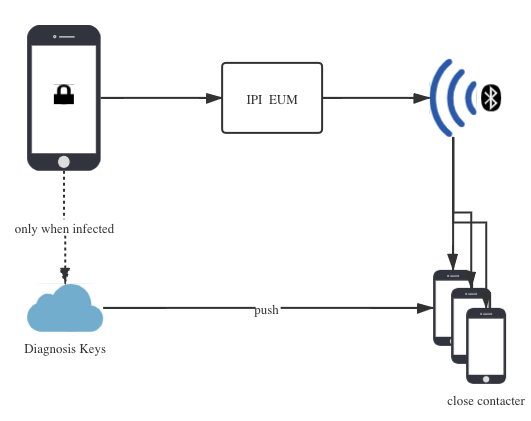
\includegraphics[width=0.7\linewidth]{figure/judge}
	\caption{The 3 Code Interaction}
	\label{fig:fig1}
\end{figure}


\subsubsection{Mathematic Detail}
% \textbf{HMAC}

% HMAC definition is taken from RFC 2104:
% $$HMAC(K,m)=H((K'\oplus opad)||H(K'\oplus ipad) || m)$$

% where $H$ is a cryptographic hash function, $m$ is the message to be authenticated, $K$ is the secret key, $K'$ is a block-sized key derived from the secret key.


\textbf{HKDF}

HKDF \cite{briefxip3322b}designates the HKDF function as defined by IETF RFC 5869, using the SHA-256 hash function: 
$$Output\leftarrow HKDF(key,Salt, Info, OutputLength)$$

\textbf{AES}

AES \cite{gueron2020flexible}designates the encryption of a single AES-128 block
$$Output\leftarrow AES_{128}(Key,data)$$

\textbf{CRNG}

The CRNG \cite{datcu2020chaos}function designates a cryptographic random number generator: 
$$Output\leftarrow CRNG(OutputLength)$$

\textbf{Tracking Interval Number}

Tracking Interval Number(TIN) offers a number for each 15 minute period that’s shared between all devices participating in the protocol. These time windows are derived from timestamps in Unix Epoch Time. TIN is encoded as a 32-bit unsigned little-endian value.

$$TIN(timestamp)\leftarrow timestamp/(60\times 15)$$

\textbf{PREKRollingPeriod}

PREKRollingPeriod(PREKP) is the duration determining the duration a Periodic Rolling Encryption Key is valid(in multiples of 15 minutes). In our protocol, PREKP is defined as 96(quarter hours), achieving a key validity of 24 hours. 

\textbf{Periodic Rolling Exposure Key}

When setting up the device for exposure detection, the first Periodic Rolling Exposure Key(PREK) is generated on the device and associated with an TIN , corresponding to the time from which the
key is valid. That value is aligned with the PREKP and is derived as follows: 

$$i\leftarrow \lfloor TIN(time_{keygen})/PREKP\rfloor \times PREKP$$

The devices generate the 16-byte Temporary Exposure Key as follows: 
$$PREK_i\leftarrow CRNG(16)$$

The key is securely stored along with $i$. At the end of every PREKRollingPeriod, a new key is generated. 

\textbf{Interval Proximity Identifier Key}

Interval Proximity Identifier Key(IPIK) is derived from the Periodic Rolling Exposure Key and is used in
order to derive the Rolling Proximity Identifiers\cite{hirmer2020techniques}. 
$$IPIK_i\leftarrow HKDF(PREKP_i,NULL,UTF8("IPIkey"), 16)$$

\textbf{Interval Proximity Identifier}

Interval Proximity Identifiers are broadcast in Bluetooth payloads with privacy-preserving functionalities.

the protocol generates a new IPI as long as Bluetooth metadata changed.

$$IPI_{i,j}\leftarrow AES_{128}(RPIK_i,0||TIN_j)$$

Where the length of $0||TIN_j$ is 128bit.

\textbf{Encrypted User Metadata Key}
The Encrypted User Metadata Keys(EUMK) are derived from the Periodic Rolling Exposure Keys in order to encrypt additional metadata.
$$EUMK_i\leftarrow HKDF(PREK_i,NULL,UTF8("EUMKey"), 16)$$

\textbf{Encrypted User Metadata}
The Encrypted User Metadata(EUM) is data encrypted along with the Interval Proximity Identifier, and can only be decrypted later if the user broadcasting it tested positive and reveals their Periodic Rolling Exposure Key\cite{keselman2020homomorphic}. 
$$EUM_{i,j}\leftarrow AES_{128}-CTR(EUMK_i,IPI_{i,j},BLEMetadata)$$


\subsubsection{Inter-Device Communication}
In our protocol, the client uses Bluetooth low energy beacon to transmit Bluetooth payload containing Encrypted User Metadata and Interval Proximity Identifier to other proximate receivers. Mobile phone offers API for WeChat to use Bluetooth Data transmission.

Similar to WiFi device discovery, the protocol is based on advertising\cite{tang2020privacy}, a.k.a. Bluetooth payloads that our device sends out to anyone within reach, and scanning, which is receiving and reading other devices advertisements.

No connection between devices is ever made: all devices will throw messages out in the air and read whatever comes in.

\section{Discussion}
\subsection{Security}
In our protocol, only infector's Periodic Rolling Exposure Key will upload to the cloud server. So it is impossible for the server to collect uninfected privacy data. For infector, their exposed Periodic Rolling Exposure Key will leak little privacy as the key schedule is fixed and defined by operating system components, preventing applications from including static or predictable information that could be used for tracking. 

When the user receives others' Interval Proximity Identifiers, a Periodic Rolling Exposure Key is required to correlate between these IPIs. Because the IPIs vary within a short period. The probability of cracking the  IPI  is negligible, which reduces the risk of privacy loss from broadcasting the identifiers. Without the knowledge of Periodic Rolling Exposure Keys, it's computationally infeasible for an attacker to find a collision on an Interval Proximity Identifiers. This prevents a wide range of replay and impersonation attacks. 

When reporting Diagnosis Keys, the correlation of Interval Proximity Identifiers by others is limited to 24 hour periods due to the use of Periodic Rolling Exposure Keys that change daily. The server must not retain metadata from clients uploading Diagnosis Keys(Periodic Rolling Exposure Keys of infectors) after including those key in the aggregated list of Diagnosis Keys per day.

% , which can not infer the metadata, so the cloud server can not read person's information. The Metadata Tracking Code or Temporary Exposure Key $tek$ are stored in the users' devices, which may contain some privacy information, It can not be acquired from the $aemk$ as we use $tek$ generate $aemk$ with $HKDF$. A government of this country has developed a tracking tool using this set of APIs. On the server side, administrators cannot know which other users a healthy user has contacted with—the administrator can only do so for diagnosed patients.

% Also, the uploaded information does not include geographic location information and is strictly limited to the use of Bluetooth low energy beacons. The Heartbeat Tracking Code is bound to the Periodic Tracking Code. Even if there is a confirmed patient, the calculation of the diagnostic Heartbeat Tracking Code uploaded by it is only performed on other users' mobile phones, not on the server side.



\subsection{Properties and functionalities}
As every mobile phone is equipped with Bluetooth low-power beacon, the protocol development is possible. The Bluetooth data transmission transmits 16 Byte data each time, the total data received is not supposed to exceed 1MB each day. It will cost no more than 20MB in a quarantine period to take up the phone's storage. Besides, the power consumption can be little, so it will not reduce the user's device battery life remarkably.

The government can pin the location of infector through distributed awareness system, which collects data of those who have ever been inclosed with infectors. With these data, it's easy to draw the movement trajectory of infector in the short term. The WeChat also offers location history. Due to the Catastrophic consequences, COVID-19 has caused, most people will be willing to accept this level of surveillance to prevent the virus from spreading temporarily. Besides, Statistical data can be obtained from Wechat client as people need to refresh their health data periodically. 

% Information transferred between different parties is performed through bluetooth, But the data is encrypted. 

% Due to the setting of Bluetooth broadcast and scanning intervals, and the length of each Heartbeat Tracking Code is only 32 bytes, this set of technology implementation is also more power-saving and storage space-saving\cite{aiello2009bluetooth}. Overall, its power consumption should not be very impressive, at least it will not reach the exaggerated Chengdu. Of course, the specific broadcast and scan interval can be set by the operator of the tracking tool.

\section{Conclusion}
In this article, we propose a privacy-preserving protocol based on BluetoothEncrypted data sharing and verified its security and functionalities. The server only records the diagnosis key of the positive infected person and does not get privacy information from it. The data exchange based on Bluetooth low energy beacon is high-efficiency and low-power. It is easy to built taking WeChat Health Code App as frontend. To a certain extent, it can play the role of epidemiological traceback and infection risk alert.
\bibliography{wpref}

\end{document}
